\section{Results}
\label{sec:results}

\subsection{Preliminary findings}

To find the best model-fit to the station data for the historical period a 9-point grid around the grid closest to the station is used. The maximum precipitation value for each time step is chosen out of the 9 grid points. This is done to minimize the risk of missing an modelled event next to the station grid-point. An event modelled at a certain grid-point might as well happen at the grid-point next to it. To evaluate if this grid selection is better than choosing the grid-point closest to the stations the absolute average difference between the station values and the model values for all durations is calculated for both the 1 grid-procedure and the 9-grid-procedure. If the difference is 0 it means the modelled values are equal to the station-values.  

\begin{table}
\begin{tabular}{ c c c c }

Duration & 1grid & 9grid & diff 1g-9g \\
2 & 2.93 & 8.22 & -5.30 \\
5 & 5.62 & 8.54 & -2.92 \\
10 & 7.86 & 8.93 & -1.07 \\
20 & 10.23 & 9.66 & 0.57 \\
25 & 11.04 & 9.96 & 1.08 \\
50 & 13.71 & 11.19 & 2.52 \\
100 & 16.68 & 12.73 & 3.95 \\
200 & 20.02 & 14.58 & 5.44
\end{tabular}
    \label{grid}
\end{tabular}
\caption{Grid selection. Positive difference: 9grid is better. Negative: 1grid is better}
\end{table}

As displayed is Table \ref{grid} the 9grid-selection outperforms the regular 1grid-selection on the larger return periods, while it is the opposite for smaller return periods.
\textbf{Whys is this the case?}

\subsection{Surrounding grid points Blindern station}

It turned out that the "1grid" approach underestimated the returnvalues, while the "9grid" approach overestimated them. I have calculated the mean difference between the station Blindern and the individual gridpoints surrounding the station to check if any of the gridpoints have particular large impact on the maximum value chosen per time step in the "9g" analysis. The gridpoint to the south and south-west where further away from the station than the other directions by a huge margin. For some return periods the difference where more than twice as large as the smallest differnece for that return period. These directions may affect the overall "9grid" method too much.   

In the "retlev" values in "IDF ECE Blindern 9grid.csv" is smaller for almost all directions and return periods. This is a mismatch with the resulting figures from the 9grid selection method. For all return periods in these figure the Blindrn return values are alot higher for the modeled data over the station data. So why are all return values from the grid points around blindern lower than the station? something is incorrect.

The individual 9g grid points have very lov mean return values for all return periods compared to the first 9g method. Should be the same. 

\subsection{9grid mean vs max method}
Previously the selection method was based on choosing the maximum value per time-step out of the nine gridpoints, forming a one-dimensional timeseries. Then the annual maxima was extracted for each duration. This approach was designed to maximize the chance of capturing an extreme event in close proximity to the station. As discussed above (?) this method appears to "optimize" the modeled precipitation and hence overestimate the return values. Retunvalues for all stations and almost all durations are within the 95 percentile of the station-based retunvalues for the larger returnperiods. This is not surprising given the enormous confidence interval in the largest retunperiods at up to around 200 mmm for the largest durations for some stations. For the smaller returnperiods like 2 and 5 years the method is outside the 95 percentile of the station-based returnvalues. Here the confidence interval is of coarse noticeably smaller. \textbf{make sure its even relevant to comapre this against the confidence interval to the stat based values. Justify it somewhere}.  

The two "new"/other 9-grid based selection methods are built differently. Now the annual maximum value for each of the nine  gridpoints for each duration is extracted directly and put into a 3x3 matrix. Either maximum ($MAX$) or mean ($MEAN$)values of the nine is then calculated per duration to give a one-dimensional data series. The $MAX$ alternative is designed to be a less aggressive optimisation of the annual maximum values around the station compared to the other nine-grid maximum selection method \textbf{make a name for this one as well!}. The  $MAX$ maximization method is possibly closer to the real world compared to the \textbf{$XXX$} method. Extracting maximum value for each timestep out of the nine gridpoints might be artificial in one way, since the annual maxima for any duration may be composed from different locations. The $MAX$ method is on the other hand more realistic in the sens that the annul maxima for certain year always origins from one gridpoint. 

\textbf{Here (or later) you can discuss what the station is actually representing. It might be that the $XXX$ method is very representative for the area in general. It would be interesting to check how the station-based IDF curves compares to observations. If these curves are underestimating the observations $XXX$ might be very well suited to represent the overall conditions fr extreme precipitation in the area.}

The resulting $MEAN$ method provides very similar returnvalues to the $1GRID$ method for all stations and all durations. For short returnperiods like 2 or 5 years the returnlevels are close to identical to the $1GRID$ method for all durations and stations, while for the larger returnperiods like 100 or 200 years the $MEAN$ method yields slightly smaller returnvalues for durations up to around 3 hours. This difference appears a smoother inclination of returnvalues compares to the very flat evolution of the $1GRID$ returnvalues for durations between 90 minutes and 3 hours. Out of all the methods the $1GRID$ and the $MEAN$ methods are clearly producing the smallest returnlevels for all stations and durations, and they are consequently smaller compared to the station-based values. Both the $MEAN$ and the $1GRID$ have almost identical returnvalues for all durations on short returnperiods for stations 18701 Blindern, 18320 Hausmansgate and 18270 Vestli. 

\begin{figure}
    \centering
    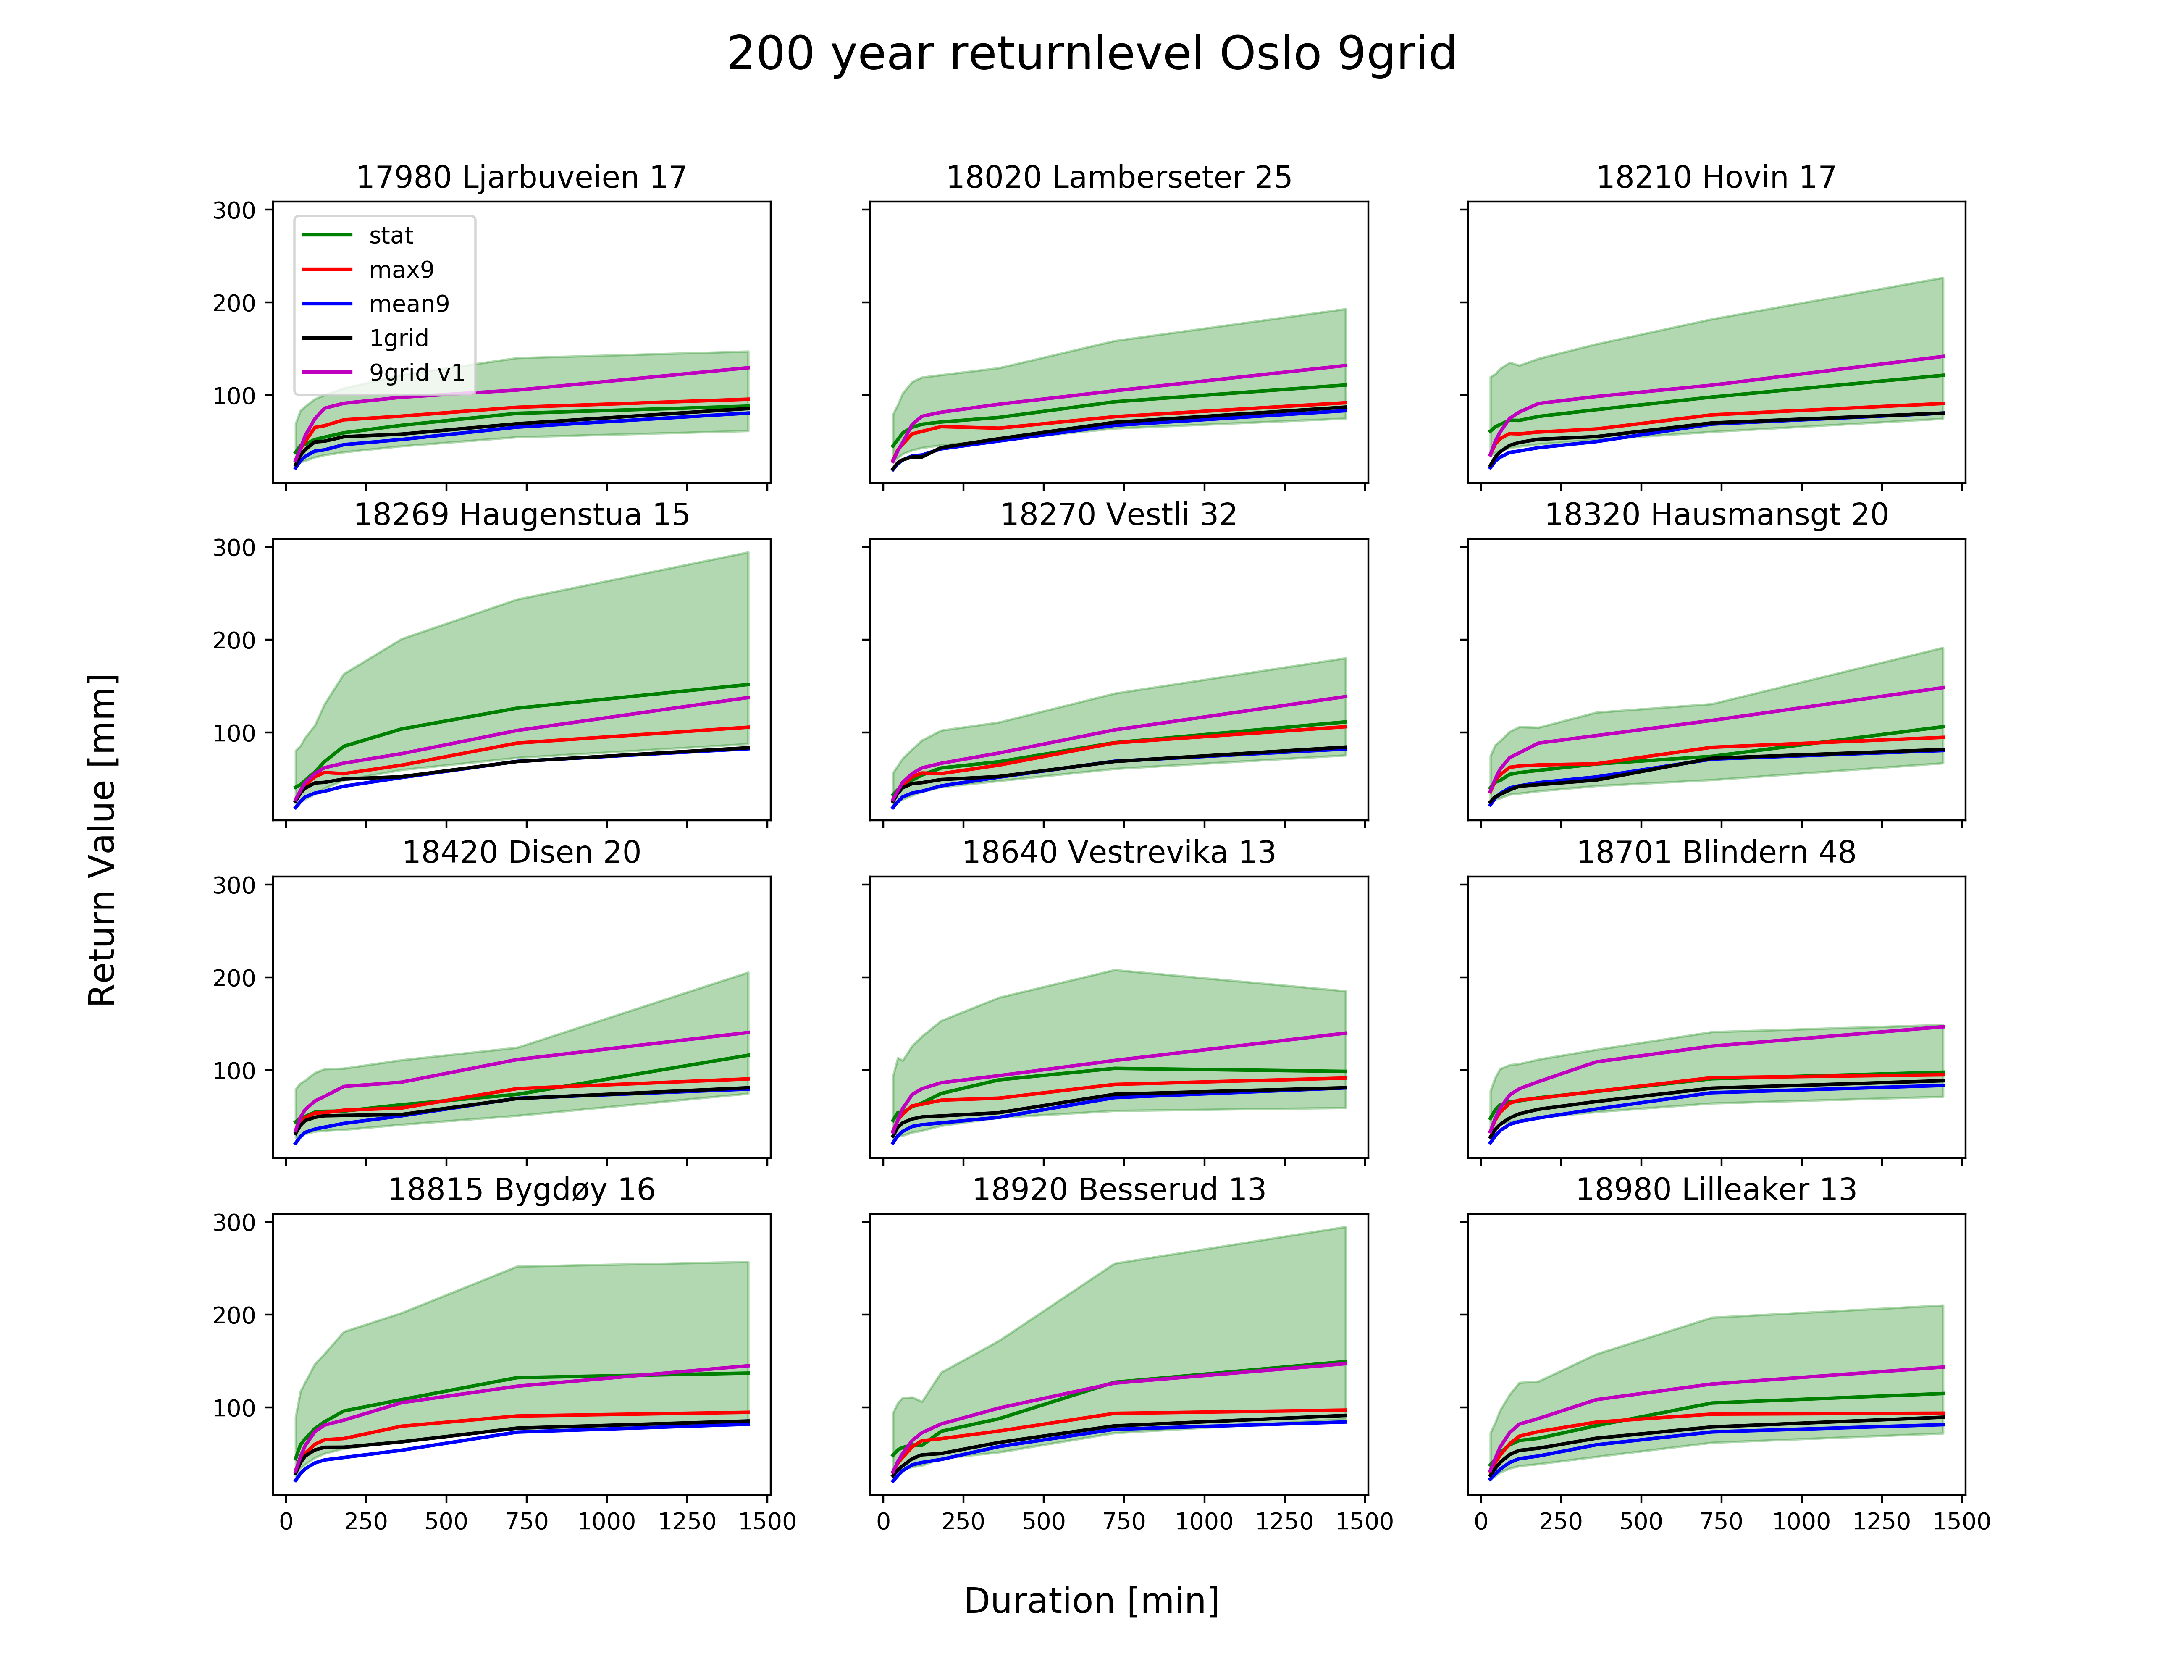
\includegraphics[scale=0.4]{figures/200_retper_ECE_1985_compare.png}
    \caption{Example figure. This is what I am talkin about
    \cite{lind_arome}}
    \label{fig:arome_domain}
\end{figure}

For most stations the $MAX$ method 



Even though we (I and Malte) agreed on not using the distance between the curves as any measure, it must be said that the "ax9" method now gives far better overall results compared to the stat.